\documentclass[11pt,a4paper]{article}

\usepackage[margin=2.2cm]{geometry}
\usepackage[T1]{fontenc}
\usepackage{lmodern}
\usepackage{microtype}
\usepackage{booktabs}
\usepackage{tabularx}
\usepackage{array}
\usepackage{xcolor}
\usepackage{graphicx}
\usepackage{float}
\usepackage{enumitem}
\usepackage{titlesec}
\usepackage{fancyhdr}
\usepackage{listings}
\usepackage{tikz}
\usetikzlibrary{arrows.meta,positioning,shapes.geometric,fit,calc}
\usepackage[hidelinks]{hyperref}

\definecolor{ink}{HTML}{1B2A3A}
\definecolor{teal}{HTML}{0F766E}
\definecolor{soft}{HTML}{E6F2F1}
\definecolor{warn}{HTML}{B45309}
\definecolor{codebg}{HTML}{F4F6F8}

\titleformat{\section}{\Large\bfseries\color{ink}}{\thesection}{0.8em}{}
\titleformat{\subsection}{\large\bfseries\color{teal}}{\thesubsection}{0.6em}{}
\setlist{itemsep=2pt,topsep=4pt}
\renewcommand{\arraystretch}{1.25}

\lstset{basicstyle=\ttfamily\footnotesize,backgroundcolor=\color{codebg},
  frame=none,breaklines=true,columns=fullflexible,xleftmargin=4pt,
  aboveskip=6pt,belowskip=6pt}

\pagestyle{fancy}
\fancyhf{}
\lhead{\small\color{gray}Private Network Service Platform}
\rhead{\small\color{gray}Team 1 --- Computer Networks Capstone}
\cfoot{\small\thepage}
\renewcommand{\headrulewidth}{0.3pt}

\newcommand{\cmd}[1]{\texttt{#1}}

\begin{document}
\sloppy

% ------------------------------------------------------------------ title
\begin{titlepage}
\centering
\vspace*{3cm}
{\color{teal}\large COMPUTER NETWORKS CAPSTONE\par}
\vspace{0.6cm}
{\color{ink}\Huge\bfseries Private Network Service Platform\par}
\vspace{0.4cm}
{\Large Private DNS, HTTPS edge, load balancing and resilience\\ on a four-Mac LAN\par}
\vspace{1.5cm}
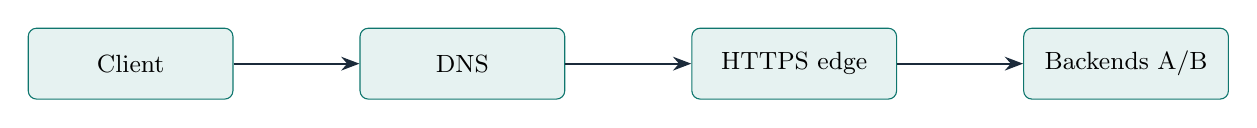
\begin{tikzpicture}[node distance=1.6cm,
  box/.style={draw=teal,fill=soft,rounded corners=3pt,minimum width=2.6cm,minimum height=0.9cm,font=\small}]
  \node[box] (c) {Client};
  \node[box,right=of c] (d) {DNS};
  \node[box,right=of d] (e) {HTTPS edge};
  \node[box,right=of e] (b) {Backends A/B};
  \draw[-{Stealth},thick,ink] (c)--(d);
  \draw[-{Stealth},thick,ink] (d)--(e);
  \draw[-{Stealth},thick,ink] (e)--(b);
\end{tikzpicture}
\vfill
{\large Team 1 \quad$\cdot$\quad Domain \texttt{team1.test}\par}
\vspace{0.3cm}
{\normalsize Phase 1 and Phase 2 final report \quad$\cdot$\quad 23 November 2026\par}
\vspace{2cm}
\end{titlepage}

\tableofcontents
\newpage

% ------------------------------------------------------------------ 1
\section{Introduction and Objectives}

We built a small but complete private service platform on four MacBooks
connected to one Wi-Fi network. A client looks up \cmd{app.team1.test} on our
own DNS server, connects to our own HTTPS edge with a certificate issued by our
own certificate authority, and is load-balanced to one of two backend
services. Phase~2 then made every layer survive a failure and secured the
backends.

\paragraph{Objectives.}
\begin{itemize}
  \item \textbf{Phase 1:} private LAN, private DNS zone, HTTPS with a trusted
        private CA, round-robin load balancing, HTTP caching, packet-level
        proof in Wireshark, and documented failure behaviour.
  \item \textbf{Phase 2:} backup DNS (Ext~A), short TTL (Ext~B), backend
        firewall isolation (Ext~C), backend high-availability failover
        (Ext~D), a standby edge with DNS cutover (Ext~E), and a structured
        fault-diagnosis method (Ext~F).
  \item \textbf{Repeatability:} every step scripted from one shared
        \cmd{config.env}, with per-Mac automated tests and a single
        \cmd{demo.sh} that runs the 11-step demonstration.
\end{itemize}

% ------------------------------------------------------------------ 2
\section{System Architecture}

\subsection{Roles and addresses}

\begin{table}[h]
\centering
\begin{tabularx}{\textwidth}{l l X l}
\toprule
\textbf{Mac} & \textbf{IP (demo LAN)} & \textbf{Role} & \textbf{Ports} \\
\midrule
Mac 1 & 10.128.139.224 & Primary DNS (dnsmasq), client & UDP/TCP 53 \\
Mac 2 & 10.128.139.225 & nginx HTTPS edge, TLS termination, load balancer & TCP 443 \\
Mac 3 & 10.128.139.70  & Backend A; standby edge (Ext E); pf firewall (Ext C) & TCP 3001, 443 \\
Mac 4 & 10.128.139.68  & Backend B; backup DNS (Ext A); main test client & TCP 3002, UDP 53 \\
\bottomrule
\end{tabularx}
\caption{Machine roles. All addresses come from \cmd{config.env}; changing one line there re-targets every script.}
\end{table}

\subsection{Topology}

\begin{figure}[H]
\centering
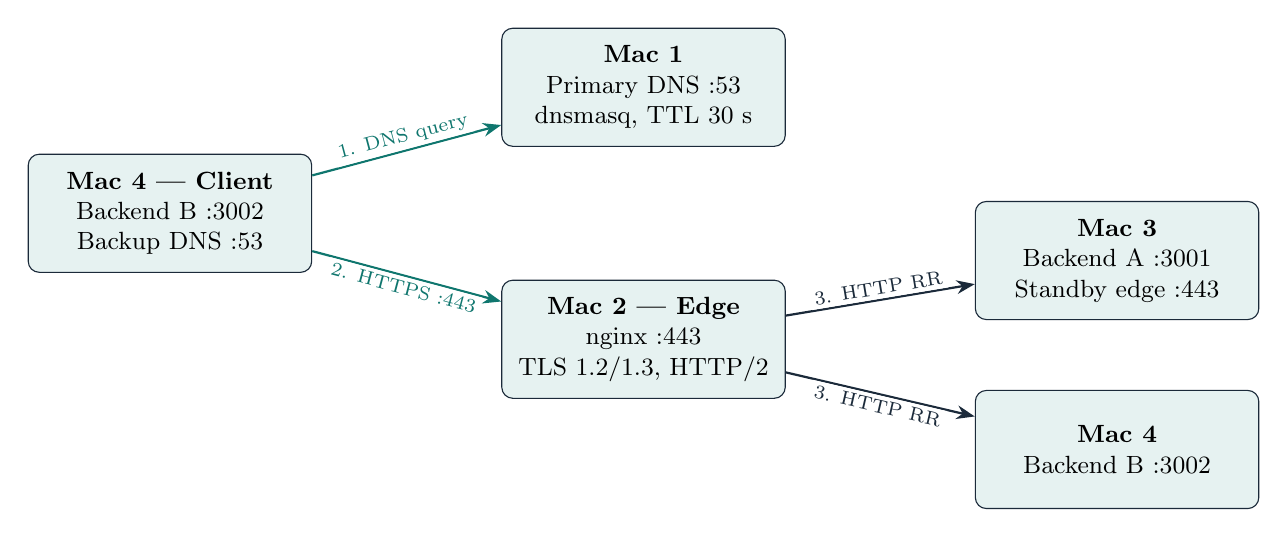
\begin{tikzpicture}[
  node distance=1.2cm and 1.6cm,
  mac/.style={draw=ink,fill=soft,rounded corners=4pt,align=center,
              minimum width=3.6cm,minimum height=1.5cm,font=\small},
  lbl/.style={font=\scriptsize,fill=white,inner sep=1.5pt},
  arr/.style={-{Stealth},thick}]
  \node[mac] (m4) {\textbf{Mac 4 --- Client}\\Backend B :3002\\Backup DNS :53};
  \node[mac,right=2.4cm of m4,yshift=1.6cm] (m1) {\textbf{Mac 1}\\Primary DNS :53\\dnsmasq, TTL 30 s};
  \node[mac,right=2.4cm of m4,yshift=-1.6cm] (m2) {\textbf{Mac 2 --- Edge}\\nginx :443\\TLS 1.2/1.3, HTTP/2};
  \node[mac,right=2.4cm of m2,yshift=1.0cm] (a) {\textbf{Mac 3}\\Backend A :3001\\Standby edge :443};
  \node[mac,right=2.4cm of m2,yshift=-1.4cm] (b) {\textbf{Mac 4}\\Backend B :3002};
  \draw[arr,teal] (m4) -- node[lbl,above,sloped]{1. DNS query} (m1);
  \draw[arr,teal] (m4) -- node[lbl,below,sloped]{2. HTTPS :443} (m2);
  \draw[arr,ink] (m2) -- node[lbl,above,sloped]{3. HTTP RR} (a);
  \draw[arr,ink] (m2) -- node[lbl,below,sloped]{3. HTTP RR} (b);
\end{tikzpicture}
\caption{Request path. The firewall on each backend admits only the two edge IPs.}
\end{figure}

\subsection{DNS zone}
\begin{tabularx}{\textwidth}{l l X}
\toprule
\textbf{Name} & \textbf{Record} & \textbf{Notes} \\
\midrule
\cmd{app.team1.test} & A $\to$ \cmd{APP\_TARGET\_IP} & Mac~2 normally; Mac~3 during Ext~E cutover. TTL 30\,s \\
\cmd{api.team1.test} & A $\to$ same & Covered by the same certificate (SAN) \\
other \cmd{*.team1.test} & NXDOMAIN & \cmd{local=/team1.test/} keeps the zone private \\
public names & forwarded & to 8.8.8.8, so Internet access still works \\
\bottomrule
\end{tabularx}

% ------------------------------------------------------------------ 3
\section{Phase 1 Implementation}

\subsection{Task A --- Private LAN}
All four Macs join one Wi-Fi network (one broadcast domain, one /24 subnet).
\cmd{evidence/01-lan/} holds each Mac's interface details and a full ping
matrix. When the network changed during testing (10.202.54.x $\to$
10.128.139.x), only \cmd{config.env} had to be edited.

\subsection{Task B --- Private DNS (Mac 1)}
\cmd{dns/start-dns.sh} generates a dnsmasq configuration from
\cmd{config.env}:
\begin{lstlisting}
address=/app.team1.test/10.128.139.225
address=/api.team1.test/10.128.139.225
local=/team1.test/          # never forward our zone
local-ttl=30                # answers carry TTL 30 s
server=8.8.8.8              # everything else is forwarded
log-queries
log-facility=-              # logs to the terminal (macOS would hide them in syslog)
\end{lstlisting}
Clients are pointed at it with \cmd{dns/set-client-dns.sh set}. We learned
that \cmd{dig} talks to the server directly, while \cmd{curl} and browsers go
through macOS's \cmd{mDNSResponder} cache, so the two can disagree for up to
one TTL.

\subsection{Task C --- Backend services (Mac 3, Mac 4)}
\cmd{backend.py} is one Python HTTP server, started twice with
\cmd{BACKEND\_NAME=A BACKEND\_PORT=3001} and \cmd{B/3002}. It serves
\cmd{/} (an HTML page), \cmd{/api/status} (JSON, \cmd{Cache-Control: no-store})
and \cmd{/api/cache}. Every response carries \cmd{X-Backend: A|B} so load
balancing is visible from the client.

\subsection{Task D --- nginx edge and load balancing (Mac 2)}
\cmd{nginx-script.sh start} writes the nginx configuration and starts it:
\begin{lstlisting}
upstream backends {
    server 10.128.139.70:3001 max_fails=1 fail_timeout=10s;   # Backend A
    server 10.128.139.68:3002 max_fails=1 fail_timeout=10s;   # Backend B
}
server {
    listen 443 ssl;  http2 on;
    ssl_protocols TLSv1.2 TLSv1.3;
    location / {
        proxy_pass http://backends;
        proxy_next_upstream error timeout http_502 http_503;
        proxy_next_upstream_tries 2;
        proxy_connect_timeout 2s;  proxy_read_timeout 5s;
        add_header X-Edge mac2-primary;  add_header X-Upstream $upstream_addr;
    }
}
\end{lstlisting}
The default algorithm is round-robin; the client sees
\cmd{X-Backend: A, B, A, B}. We removed upstream \cmd{keepalive} because
reused idle connections skewed the order after a restart.

\subsection{Task E --- HTTPS with a private CA (Mac 2)}
\cmd{mac2-certs.sh} creates the \emph{Team1 Local CA} (valid to 2036) and a
server certificate: RSA 2048, 365 days, SAN \cmd{app.team1.test} and
\cmd{api.team1.test}, Extended Key Usage \cmd{serverAuth}. Each client
trusts the CA once (Keychain plus a CA bundle in \cmd{\textasciitilde/.curlrc},
since macOS's LibreSSL curl does not always read the Keychain). After that,
\cmd{curl https://app.team1.test} and Safari work with \textbf{no warnings and
no \cmd{-k}}. TLS 1.2 and TLS 1.3 both negotiate, and HTTP/2 is selected via
ALPN.

\subsection{Task F --- HTTP caching}
\cmd{/api/cache} returns an identical body on both backends with
\cmd{Cache-Control: public, max-age=60} and a content-hash
\cmd{ETag: "512fd8b2..."}. A conditional request with
\cmd{If-None-Match} gets \cmd{304 Not Modified} and no body, whichever
backend answers, because the ETag depends only on the content.

\subsection{Task G --- Wireshark evidence}
\cmd{./demo.sh capture} records the client's traffic with the filter
\cmd{(udp port 53 and host <DNS>) or (tcp port 443 and host <edge>)}, and
\cmd{./demo.sh 6} walks through it with \cmd{tshark}:

\begin{table}[h]
\centering
\begin{tabularx}{\textwidth}{l l X}
\toprule
\textbf{Layer} & \textbf{Display filter} & \textbf{What we show} \\
\midrule
DNS (L7/UDP) & \cmd{dns} & Query \cmd{A app.team1.test}, answer with the edge IP, TTL 30 \\
TCP (L4) & \cmd{tcp.flags.syn==1} & SYN, SYN-ACK, ACK to port 443 \\
TLS 1.2 & \cmd{tls.handshake.type==11} & Certificate sent in clear: issuer \emph{Team1 Local CA}, SAN, validity \\
TLS 1.3 & \cmd{tls.handshake} & Certificate is encrypted; only ClientHello/ServerHello visible \\
HTTP & \cmd{tls.record.content\_type==23} & Application Data only --- the HTTP request is encrypted \\
\bottomrule
\end{tabularx}
\caption{Packet-level proof of each layer.}
\end{table}

% ------------------------------------------------------------------ 4
\section{Phase 2 Extensions}

\subsection{Ext A --- Backup DNS (Mac 1 + Mac 4)}
Mac~4 runs the same \cmd{start-dns.sh} with the same records. The client
lists both servers (Mac~1 first, Mac~4 second). When dnsmasq on Mac~1 is
stopped, \cmd{dig app.team1.test} still answers, with
\cmd{;; SERVER: <Mac 4>\#53}. macOS retries the second resolver after a
timeout; it is failover, not load sharing.

\subsection{Ext B --- Short TTL and resolver caching}
\cmd{DNS\_TTL=30} becomes dnsmasq's \cmd{local-ttl}. When the record is
changed on the server, \cmd{dig} shows the new IP immediately, but the
application keeps using the cached one until the TTL expires. A short TTL
makes changes take effect quickly at the cost of more DNS queries.

\subsection{Ext C --- Backend isolation with pf (Mac 3, Mac 4)}
\cmd{firewall/backend-firewall.sh apply} loads rules into a pf anchor
\cmd{com.apple/team1-backend}:
\begin{lstlisting}
pass  quick on lo0
pass  in quick proto tcp from 10.128.139.225 to any port 3001 keep state  # primary edge
pass  in quick proto tcp from 10.128.139.70  to any port 3001 keep state  # standby edge
block drop in quick proto tcp from any to any port 3001                   # everyone else
\end{lstlisting}
The edge reaches the backend; a client going directly to \cmd{:3001} times
out (silent drop). We had to fix two macOS-specific issues: an anchor is only
evaluated if it sits under \cmd{com.apple/*}, and \cmd{on any} is not valid pf
syntax. \cmd{remove} flushes the anchor and disables pf only if it was off
before. This mirrors AWS security groups that accept traffic only from the
load balancer.

\subsection{Ext D --- Backend high availability (Mac 2)}
With \cmd{max\_fails=1 fail\_timeout=10s} and \cmd{proxy\_next\_upstream},
a request that reaches a dead backend is retried on the other one and the dead
backend is skipped for 10\,s (a \emph{passive} health check). Our recorded run
(\cmd{evidence/10-ha-failover/}):

\begin{table}[h]
\centering
\begin{tabular}{l c c c}
\toprule
\textbf{Phase} & \textbf{Requests} & \textbf{HTTP 200} & \textbf{Served by} \\
\midrule
Both backends up & 6 & 6 & A=3, B=3 \\
Backend A killed & 8 & 8 & B=8 (first request 1.2\,s, retried) \\
A restarted, after 10\,s & 6 & 6 & A=2, B=4 \\
\bottomrule
\end{tabular}
\caption{The client saw no error while a backend died, and recovery needed no configuration change.}
\end{table}
\noindent If \emph{both} backends are down, TLS still succeeds and nginx
returns \cmd{502 Bad Gateway}; a backend that hangs gives \cmd{504}.

\subsection{Ext E --- Standby edge and DNS cutover (Mac 2 + Mac 3)}
After Ext~D the edge itself is the remaining single point of failure. Mac~2
exports its certificate and key (\cmd{mac2-export-certs.sh}), Mac~3 imports
and verifies them and runs the same \cmd{nginx-script.sh} as
\cmd{standby} (header \cmd{X-Edge: mac3-standby}). Mac~1 and Mac~4 then
re-point \cmd{app.team1.test} to Mac~3.

\begin{table}[h]
\centering
\begin{tabular}{l l l l}
\toprule
\textbf{Time} & \textbf{DNS server says} & \textbf{Client cache uses} & \textbf{X-Edge} \\
\midrule
12:12:38 & Mac 2 & Mac 2 & mac2-primary \\
12:12:40 & \textbf{Mac 3} (record changed) & Mac 2 & mac2-primary \\
12:13:07 & Mac 3 & Mac 2 & mac2-primary \\
12:13:09 & Mac 3 & \textbf{Mac 3} & \textbf{mac3-standby} \\
\bottomrule
\end{tabular}
\caption{Recorded cutover (\cmd{evidence/12-edge-cutover/}): the client switched 29\,s after the change, within the 30\,s TTL, with every request returning 200.}
\end{table}
\noindent Faster alternatives would be a floating IP with VRRP/keepalived
(about 1\,s), active-active edges, or a managed cloud load balancer.

\subsection{Ext F --- Fault diagnosis method}
\cmd{troubleshoot/diagnose.sh} checks the layers in order and stops at the
first that fails; \cmd{troubleshoot/RUNBOOK.md} lists 12 faults with their
symptom, proving command and fix.

\begin{table}[h]
\centering
\begin{tabularx}{\textwidth}{l l X}
\toprule
\textbf{Layer} & \textbf{Test} & \textbf{Typical fault it isolates} \\
\midrule
1 DNS & \cmd{dig app.team1.test} & DNS down, wrong record, client using 8.8.8.8 \\
2 IP & \cmd{ping <edge>} & Mac off the network, IP changed \\
3 TCP & \cmd{nc -vz <edge> 443} & nginx stopped (refused) or firewall (timeout) \\
4 TLS & \cmd{openssl s\_client -CAfile ...} & CA not trusted, expired cert, wrong name \\
5 HTTP & \cmd{curl -I https://app...} & 502 both backends down, 504 backend hung \\
\bottomrule
\end{tabularx}
\end{table}

% ------------------------------------------------------------------ 5
\section{Testing and Results}

Each Mac runs its own test script (\cmd{tests/test-macN.sh}); results are
saved under \cmd{evidence/test-results/}.

\begin{table}[h]
\centering
\begin{tabularx}{\textwidth}{l X c}
\toprule
\textbf{Script} & \textbf{Covers} & \textbf{Final run} \\
\midrule
\cmd{test-mac1.sh} & DNS server and client, HTTPS/LB/caching from a client, Ext A/B/C/E & passed \\
\cmd{test-mac2.sh} & Certificate, nginx config, TLS 1.2/1.3, HTTP/2, round-robin, reach to backends, failover and 502 on a private test edge & \textbf{24 / 24} \\
\cmd{test-mac3.sh} & Backend A, identical ETag, firewall rules, standby edge & passed \\
\cmd{test-mac4.sh} & Backend B, backup DNS, full client side, Task G capture & \textbf{45 / 45} \\
\bottomrule
\end{tabularx}
\caption{Automated test summary (23 November 2026).}
\end{table}

\noindent Failure scenarios we demonstrated and explained:
\begin{itemize}
  \item DNS server down $\to$ backup answers; both down $\to$ \emph{could not resolve host}.
  \item nginx down $\to$ \emph{connection refused} at TCP, even though ping works.
  \item One backend down $\to$ no visible error (retry); both down $\to$ 502.
  \item Untrusted CA $\to$ curl error 60; fixed by trusting the CA, never by \cmd{-k}.
  \item Firewall on $\to$ direct backend access times out, the edge still works.
\end{itemize}

% ------------------------------------------------------------------ 6
\section{Demonstration Plan}

\cmd{./demo.sh} detects which Mac it runs on and performs that Mac's part of
each step. \cmd{./demo.sh ready} prepares a clean starting state and
\cmd{./demo.sh check} is a pre-flight check.

\begin{table}[h]
\centering
\begin{tabularx}{\textwidth}{c X l}
\toprule
\textbf{Step} & \textbf{Shows} & \textbf{Led by} \\
\midrule
1 & Topology and IP / service inventory & all \\
2 & All machines on the private LAN (ping matrix) & all \\
3 & Resolve the private name from a client & Mac 1, Mac 4 \\
4 & HTTPS by name with no certificate warning & Mac 2, Mac 4 \\
5 & Load balancing across both backends & Mac 2, Mac 4 \\
6 & Wireshark: DNS, TCP and TLS & Mac 4 \\
7 & HTTP headers and caching (304) & Mac 3, Mac 4 \\
8 & Backend A fails, service continues (Ext D) & Mac 3, Mac 2 \\
9 & Phase 2: backup DNS, TTL, firewall, edge cutover (Ext A/B/C/E) & all \\
10 & Diagnose a fault injected by the examiner (Ext F) & all \\
11 & Lessons learned and cloud equivalents & all \\
\bottomrule
\end{tabularx}
\end{table}

% ------------------------------------------------------------------ 7
\section{Challenges and Lessons Learned}

\begin{tabularx}{\textwidth}{>{\raggedright}p{4.6cm} X}
\toprule
\textbf{Problem} & \textbf{Cause and fix} \\
\midrule
Network changed mid-project & Every script reads \cmd{config.env}; edited once, restarted DNS and nginx. \\
curl error 60 despite Keychain trust & macOS LibreSSL curl; added the CA bundle to \cmd{\textasciitilde/.curlrc}. \\
Safari rejected the first certificate & Missing \cmd{serverAuth} EKU and \cmd{api} SAN; re-issued from the same CA. \\
Load balancing order B, B, A, B & Upstream keepalive reused connections; removed. \\
Firewall rules had no effect & pf only evaluates anchors under \cmd{com.apple/*}; moved the anchor. \\
dig and curl disagree after a change & dig bypasses the OS cache; curl waits for the TTL. \\
DNS query logs missing & macOS sends dnsmasq logs to syslog; added \cmd{log-facility=-}. \\
\bottomrule
\end{tabularx}

\paragraph{Key takeaways.}
\begin{itemize}
  \item Redundancy has to exist at \emph{every} layer; removing one single point
        of failure exposes the next (backends $\to$ edge $\to$ DNS).
  \item DNS-based failover is cheap but only as fast as the TTL and client caches.
  \item TLS 1.3 hides the certificate from observers; TLS 1.2 does not.
  \item Diagnosing layer by layer turns a vague ``it doesn't work'' into one command.
\end{itemize}

\subsection*{Cloud equivalents}
\begin{tabularx}{\textwidth}{l X}
\toprule
\textbf{Our component} & \textbf{AWS equivalent} \\
\midrule
dnsmasq primary + backup, TTL 30\,s & Route 53 hosted zone (with health-checked failover records) \\
nginx edge, TLS, round-robin & Application Load Balancer \\
Standby edge + DNS cutover & Multi-AZ load balancer / DR edge \\
Backends A and B & EC2 Auto Scaling group or ECS tasks \\
pf anchor allowing only the edges & Security groups referencing the ALB's group \\
Private CA & AWS Private CA / ACM \\
\bottomrule
\end{tabularx}

% ------------------------------------------------------------------ 8
\section{Team Contributions}

\begin{tabularx}{\textwidth}{l X}
\toprule
\textbf{Member} & \textbf{Responsibilities} \\
\midrule
Mac 1 & Shared \cmd{config.env}, primary DNS (\cmd{dns/start-dns.sh}), client DNS setup, TTL and backup-DNS demos (Ext A/B) \\
Mac 2 & nginx edge and load balancer, private CA and certificates, HA failover (Ext D), certificate export for the standby edge (Ext E), per-Mac test scripts and \cmd{demo.sh} \\
Mac 3 & Backend A, pf firewall isolation (Ext C), standby edge (Ext E) \\
Mac 4 & Backend B, backup DNS (Ext A), main client, Wireshark capture (Task G), diagnosis script and runbook (Ext F), Phase 2 integration \\
\bottomrule
\end{tabularx}

\section{Conclusion}
The platform resolves a private name, serves it over trusted HTTPS, spreads
load over two backends, and keeps working when a backend, a DNS server or the
primary edge fails. Every behaviour is scripted, tested on each Mac and backed
by saved evidence and packet captures, so the whole system can be rebuilt and
demonstrated from the repository.

\end{document}
